\chapter{Szimulációs eredmények}

Az elkészült szimuláció működésének ellenőrzésére a legegyszerűbb módszer, az általa szolgáltatott eredmények vizsgálata. Helyes működés esetén az így kapott eredmények használhatóak továbbá az ismétlő protokoll pontosabb bemutatására is. Mivel egy általánosított modellt szimulálok, a tesztesetéknél a program felé elvárás az adott esethez várt általános jelleg produkálása. Ennek előzetes meghatározásához használhatjuk az elméleti bevezetőben már megismerteket, valamint  a szakirodalomban megtalálható egyéb szimulációkat, tanulmányokat \cite{briegel1998quantum}\cite{van2009system}\cite{bernardes2011rate}. A vizsgált esetekben, amennyiben nincsen másképp említve, a következő adatokat tekintettem alapértelmezésnek. 
Az összefonódott párok előállításáért felelős állomások 10$\mu s$-ként egyszerre 5 darab 0.7-es tisztaságú párt állítínak elő. Az egyes csatornákra jellemző ``csillapítási hossz'' 20km. A méréseket végző csomópontok mindkét beérkező csatorna felé 20 memória egységgel (összesen 40) rendelkeznek, valamint az egyes mérések előtt 0.98-as előírt tisztaságig tisztíttatják a párokat. Az alapértelmezetten használt tisztító protokoll egy a bevezetőben már ismertetetthez hasonló \cite{deutsch1996quantum} néhány későbbiekben javasolt változtatással \cite{briegel1998quantum}. Ennek lépései a programban teljes egészében, közelítések nélkül vannak szimulálva. Az egyes tisztítások sorrendjének meghatározásához használt alapértelmezett stratégia az ún. ``greedy bottom up '', aminek pontos leírásával majd a későbbiekben foglalkozom. Az egyes mérések elvégzése egy a későbbiekben tárgyalt fa szerű struktúra szerint történik. Az állomások közötti kommunikáció, valamint a pár szétosztás sebessége az optikai kábelekben jellemző $2 \times 10^8 \ m/s$. A vizsgált esetek teljesítményét az egységnyi idő alatt sikeresen megosztott párok számával mérem.

\section{Ismétlő protokoll és az egyszerű csatorna}

Első tesztesetnek azt vizsgáltam milyen távolság fölött kezd egyáltalán előnyt nyújtani a protokoll az ismétlő nélküli csatornával szemben. Tudván, hogy a csatorna átvitele a távolsággal exponenciálisan csökken, míg az ismétlőé csak polinomiálisan \cite{briegel1998quantum} azt várom, hogy kis távolságoknál egyszerűsége miatt a csatorna mutat jobb teljesítmény, míg egy bizonyos távolság felett az ismétlő. Szimulációval 5-500 km-es távolságig vizsgáltam az egyes esetek teljesítményét. Először azt az idealizált esetet tekintve, ahol csak a párok elvesztésével kell számolni, a tisztaságukkal nem (szétosztott párok tisztasága = 1), később a csatorna esetén a végpontokban, az ismétlőknél pedig a köztes állomásokon elvégzendő tisztítás hatását is figyelembe véve.
\begin{figure}[H]
\centering
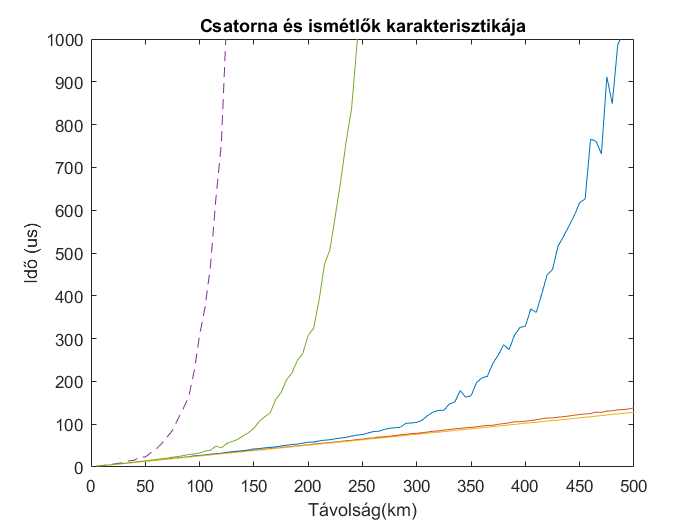
\includegraphics[width=120mm,keepaspectratio]{repvschf1}
\caption[Csatorna és ismétlők karakterisztikája 1]
{Csatorna és különböző ismétlők átvitele a távolság függvényében:\\
Az y tengelyen az egy pár megosztásához szükséges átlagos időt mérjük.\\
Lila szaggatott vonal:egyszerű csatorna.\\
zöld, kék, piros, narancs vonalak: 2, 4, 8 valamint 16, köztes létrehozó állomásból álló ismétlő rendszerek.\\
A szimuláció során kizárólag az átvitel során történő pár vesztést vizsgáltam (megosztott párok tisztasága 1-> nem kell tisztítani).\\
A csatorna és a 2 generátoros rendszer esetében a szimulációt idő előtt leállítottam a veszteségek miatt megnövekedett szükséges számítási kapacitás miatt.
}
\end{figure}
\begin{figure}[H]
\centering
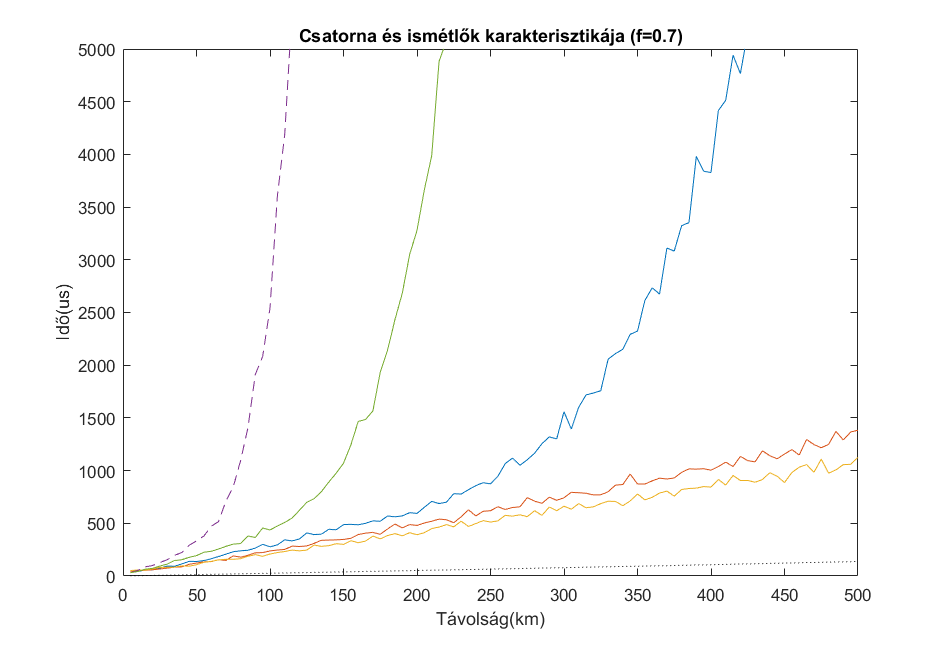
\includegraphics[width=120mm,keepaspectratio]{repvschf07}
\caption[Csatorna és ismétlők karakterisztikája 2]
{Csatorna és különböző ismétlők átvitele a távolság függvényében:\\
Az y tengelyen az egy pár megosztásához szükséges átlagos időt mérjük.\\
Lila szaggatott vonal:egyszerű csatorna.\\
Zöld, kék, piros, narancs vonalak: 2, 4, 8 valamint 16, köztes létrehozó állomásból álló ismétlő rendszerek.\\
Alsó fekete pontozott vonal: 8 köztes állomásból álló rendszer teljes tisztaság esetén.\\
A szétosztott párok ebben az esetben nem ideálisak, a tisztaságuk 0.7-es. Ennek következtében szükség van a tisztító eljárások végrehajtására. (egyszerű csatorna esetében ez a végpontokon történik.)\\
A csatorna és a 2 generátoros rendszer esetében a szimulációt itt is idő előtt leállítottam a veszteségek miatt megnövekedett szükséges számítási kapacitás miatt.
}
\end{figure}
Az egyes esetek teljesítményét az egy pár megosztásához szükséges átlagos idővel mértem (200 megosztott párból számolva).
Látható a csatorna átvitelének exponenciális romlása, valamint nagyobb távolságok esetén az ismétlő elrendezések is ezt a jelleget mutatják. Ennek oka, hogy az egyes állomásokat is exponenciálisan romló csatornák kötik össze. A protokoll fő előnye, hogy egy nagy ilyen szakasz helyett használhatunk több kisebbet. A tisztaság rontásának hatása is megfigyelhető: a teljesen tiszta esethez képest ilyenkor a tisztítás miatt több párt kell felhasználni egy tiszta pár létrehozásához a végpontok között. A görbék jellege nem változott viszont az átlagos idő nőtt.\\
Az ismétlő protokollok természetesen több erőforrást használ mint csupán egy csatorna, viszont ezzel az előzőekben nem foglalkoztam. Ennek figyelembevételre tekintettem a következő eseteket: Álljon rendelkezésre egy 8 generátoros, állomásonként 8x5 memóriaegységgel rendelkező rendszer megvalósításához szükséges erőforráshalmaz. Ebből készíthető egygenerátoros esetben egy 8-szor gyorsabb párgenerátor, valamint egyenként 8x5 pár kezelésére alkalmas végpont. Ezen logika mentén elkészíthető még 2 generátoros rendszer, 4-szer gyorsabb generátorokkal és 4x5 memóriával rendelkező állomásokkal, valamint hasonló logika alapján egy 4 és 8 generátoros rendszer is. Ezek egymáshoz képesti teljesítménye:
\begin{figure}[H]
\centering
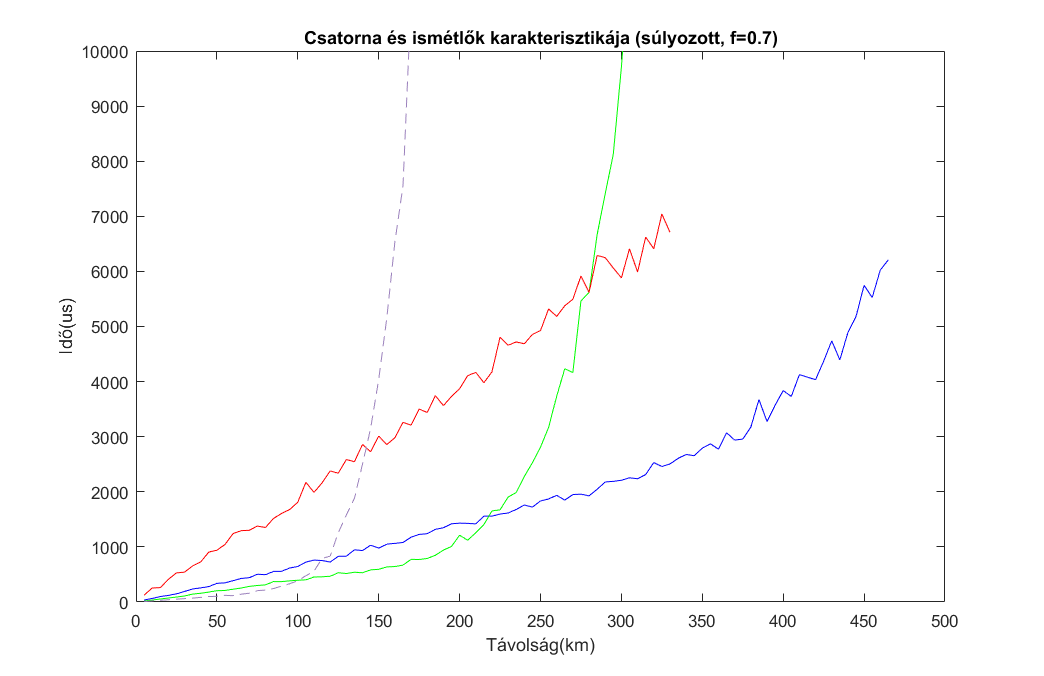
\includegraphics[width=120mm,keepaspectratio]{repvschhandicapped}
\caption[Csatorna és ismétlők karakterisztikája 2]
{Csatorna és különböző ismétlők átvitele a távolság függvényében:\\
Az y tengelyen az egy pár megosztásához szükséges átlagos időt mérjük.\\
Lila szaggatott vonal:egyszerű csatorna.\\
Zöld, kék, piros, vonalak: 2, 4, 8 köztes létrehozó állomásból álló ismétlő rendszerek.\\
A szimulációhoz szükséges idő növekedése miatt, egyes szimulációkat a páronkénti 5000 $\mu s$-os határ elérésénél leállítottam.\\
Az eredményekből látszik, hogy adott erőforrásmennyiség esetén távolságtól függően változik a leggazdaságosabb elrendezés.
}
\end{figure}
Előzetes várakozásoknak megfelelően kis távolságoknál egyszerűsége miatt a csatorna teljesít jobban egészen addig amíg az exponenciális jellegéből származó  veszteségek egy kritikus értéket meg nem haladnak. Innentől kezdve először a 2 majd 4 szegmenses ismétlő bizonyul jobbnak. A 8 szegmenses rendszerről a korábbi eredmények jellegének ismeretében feltételezhető, hogy 500-600 km-es távolság esetén már a legjobb alternatívát nyújtja, mivel 500km-hez közelítve a 4 szegmenses elrendezés is exponenciálisan kezd romlani, viszont ezek az értékek már nem tartoznak bele a szimulált tartományba. Ettől eltekintve is látszik a protokoll előnye nagyobb távolságok esetén, ami egy másik komoly optimalizálási feladatot is felvet. Korlátozott mennyiségű erőforrás esetén az adott paraméterekhez tartozó optimális méretű rendszer és az ehhez szükséges erőforrásfelosztás meghatározását.

\section{Mérési sorrend}

A protokoll működése során fontos szerepe van az egyes mérések elvégzési sorrendjének is. A következőkben két különböző stratégiát vizsgálok. Az egyik stratégia a többi vizsgálatnál általam alapértelmezettnek használt, ahol a mérések sorrendjét egy faszerű struktúra határozza meg. Itt a hálózat tipikusan $2^n+1$ elemből áll (bár a végpontoknak csak az egyik felét használjuk). Két azonos szinten lévő csomópont között a kapcsolatot mindig a közöttük félúton lévő állomáson elvégzett mérés hozza létre. Ennek megfelelően egy egyszerű hálózatra ez a következőt jelenti:
\begin{figure}[H]
\centering
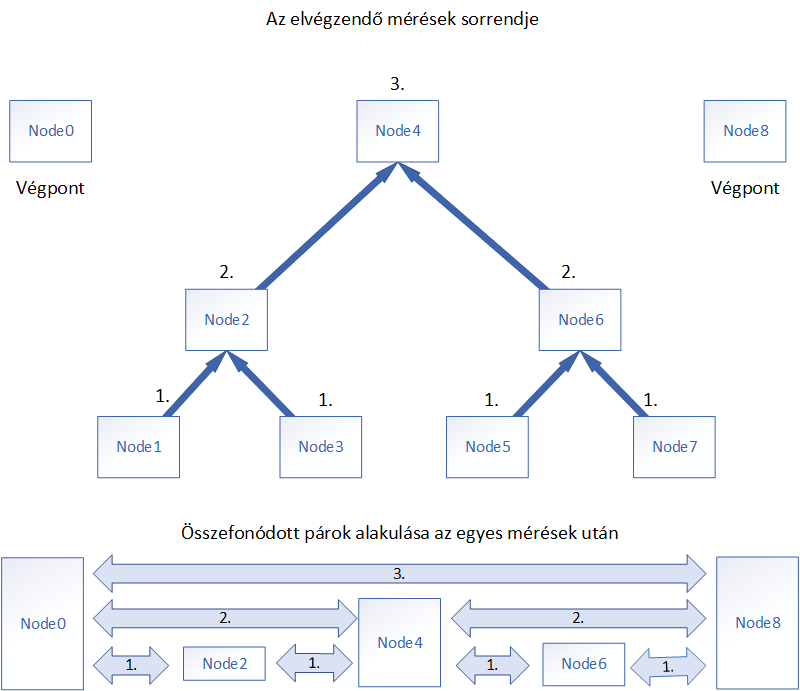
\includegraphics[width=\textwidth,keepaspectratio]{pow2tree}
\caption[Fa alapján történő mérési stratégia]{Az egyes számok a mérések elvégzési sorrendjét jelölik (feltételezzük, hogy minden állomáson rendelkezésre állnak az ehhez szükséges generátorok által küldött párok). A nyilak a sorban következő elvégzendő mérést jelölik, valamint az alsó ábrán az állomások közötti összefonódásokat.}
\end{figure}
Az elrendezésből látszik, hogy ez a stratégia akkor a leghatékonyabb, ha $2^n-1$ közbenső állomás van (+2 végponttal lesz így $2^n+1$ állomás összesen).\\
A másik vizsgált stratégiánál egyszerűen sorban végezzük el a méréseket. Ez a következőképp néz ki:
\begin{figure}[H]
\centering
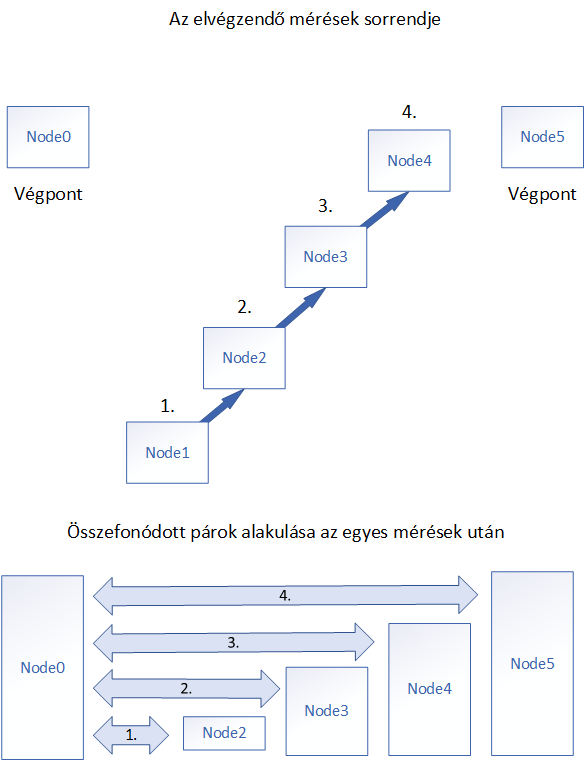
\includegraphics[width=120mm,keepaspectratio]{lintree}
\caption[Egyszerű mérési stratégia]{Az egyes számok itt is a mérések elvégzési sorrendjét jelölik (feltételezzük, hogy minden állomáson rendelkezésre állnak az ehhez szükséges generátorok által küldött párok). A nyilak a sorban következő elvégzendő mérést jelölik, valamint az alsó ábrán az állomások közötti összefonódásokat.}
\end{figure}
Ennél a második elrendezésnél a szegmensek száma közömbös az ideális hatékonyság szempontjából. A következő szimulációknál 400 km-es távolság esetén vizsgálom az alapértelmezett paraméterek mellett a fentebb bemutatott stratégiákat.
\begin{figure}[H]
\centering
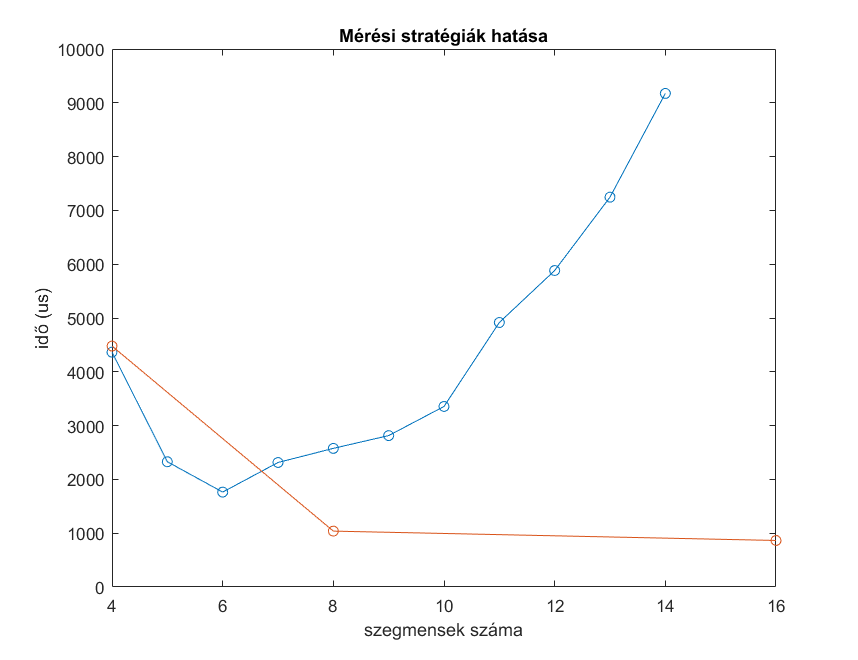
\includegraphics[width=120mm,keepaspectratio]{sorrend}
\caption[Mérési stratégiák]{A mérési stratégiák által nyújtott teljesítmények.\\
Kék vonal: egyszerű mérési stratégia\\
Piros vonal: Fa alapján történő mérési stratégia.
}
\end{figure}
Az eredményekből látszik az első elrendezés előnye. Érdekes, hogy az egyszerű stratégia esetében a rendszer a szegmensek számának növelésével lassul. Ez az állomások számával egyre növekvő klasszikus kommunikációból származó késleltetéseknek tudható be.


\section{Összefonódott pár létrehozási sebesség hatása}

A protokoll egy fontos elemét képezik az összefonódott párok generálását végző állomások. A következőkben azt vizsgáltam, miként hat az átviteli sebességre a párok létrehozási sebességének változása. A szimulációhoz használt paraméterek a következők: Az állomások mindkét irányba 10 db memóriaegységgel rendelkeznek, valamint a generáló állomások egyszerre csak 1 db összefonódott párt állítanak elő. Az egyes párok 0.7-es tisztaságúak. Az egyes adatpontok a 200 pár megosztása során gyűjtött adatok átlagai. Az így kapott eredmények:
\begin{figure}[H]
\centering
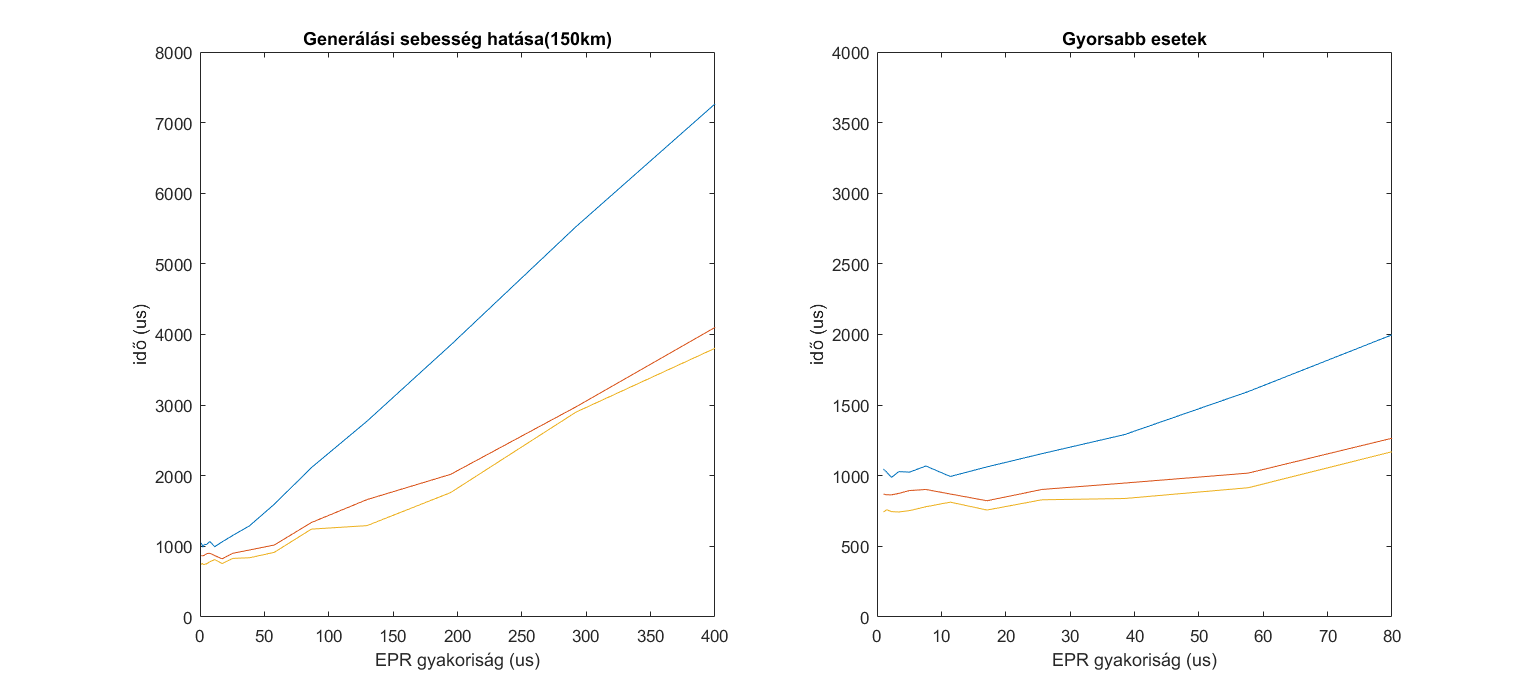
\includegraphics[width=\textwidth,keepaspectratio]{epr150}
\caption[Generálási sebesség hatása(150km)]{Generálási sebesség hatása az átviteli sebességre 150km-es szakaszon.\\
A kék,piros, sárga vonalak a 4,8,valamint 16 szegmensből álló rendszerekhez tartozó adatokat jelképezik.\\
Jobb oldalt a bal oldali grafikon kezdeti részére ráközelített kép látható.
}
\end{figure}
\begin{figure}[H]
\centering
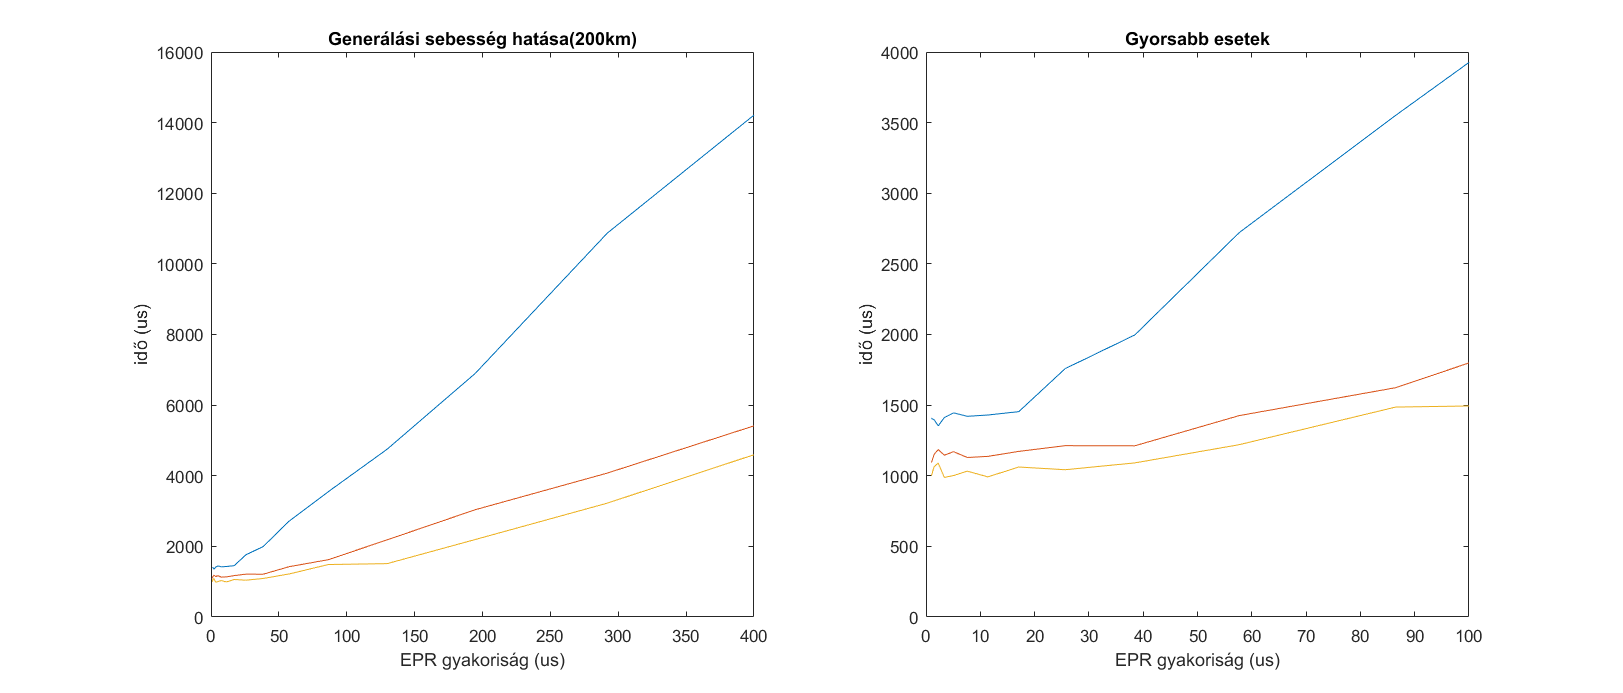
\includegraphics[width=\textwidth,keepaspectratio]{epr200}
\caption[Generálási sebesség hatása(200km)]{Generálási sebesség hatása az átviteli sebességre 200km-es szakaszon.\\
A kék,piros, sárga vonalak a 4,8,valamint 16 szegmensből álló rendszerekhez tartozó adatokat jelképezik.\\
Jobb oldalt a bal oldali grafikon kezdeti részére ráközelített kép látható.
}
\end{figure}
\begin{figure}[H]
\centering
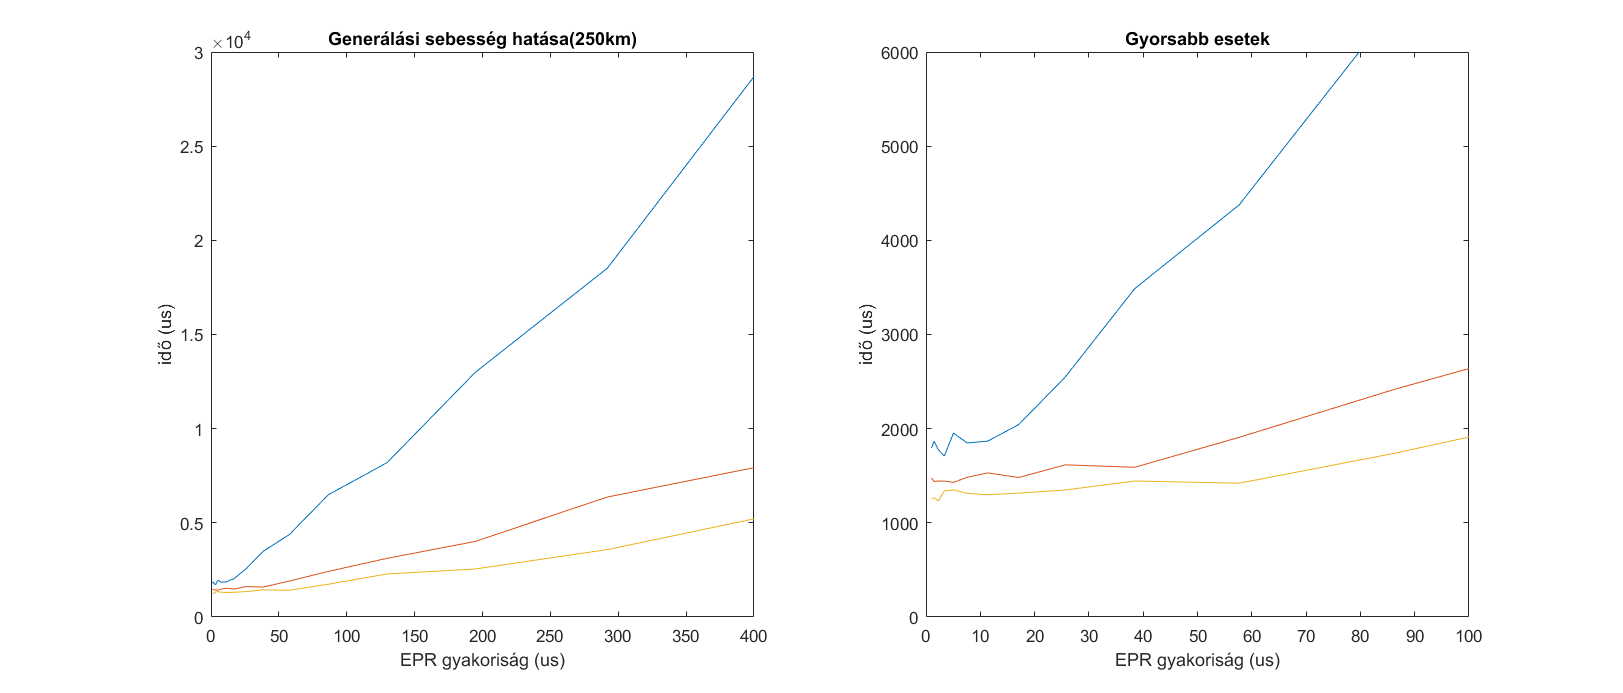
\includegraphics[width=\textwidth,keepaspectratio]{epr250}
\caption[Generálási sebesség hatása(200km)]{Generálási sebesség hatása az átviteli sebességre 200km-es szakaszon.\\
A kék,piros, sárga vonalak a 4,8,valamint 16 szegmensből álló rendszerekhez tartozó adatokat jelképezik.\\
Jobb oldalt a bal oldali grafikon kezdeti részére ráközelített kép látható.
}
\end{figure}
Figyeljük meg, hogy a nagyon gyors sebességeknél (~5-10 $\mu s$/pár alatt) már nem gyorsul tovább a rendszer. Ennek oka, hogy ennél a generálási sebességnél a generáló állomások a fogadók memóriáját már szinte folyamatosan telítve tudják tartani, így a protokoll többi részének elvégzése (mérések, egymás közti kommunikáció) adja a megosztáshoz szükséges idő jelentős részét. Lassabb sebességek esetén viszont az látszik, hogy az átvitel közel egyenesen arányos a párok generálásának sebességével. Ebben az esetben a fogadó állomások már nincsenek telítődve, így a megosztáshoz szükséges idő jelentős részét a párokra való várakozás adja.


\section{A fogadott párok tisztasága}
A fogadott párok tisztaságának is hatása van a protokoll sebességére. A tisztítóeljárásokról általánosan elmondható, hogy a művelet utáni tisztaság, valamint a tisztítás sikerességének valószínűsége is függ az elhasznált párok tisztaságától. Ebből következik, hogy minél ``koszosabbak'' a fogadott párjaink, annál többre van szükség belőlük egy megfelelően tiszta állapot előállításához. Ennek hatását vizsgáltam az alábbi szimulációs esetekkel:\\
A paraméterek az alapértelmezettek, a párok tisztaságának kivételével. Az egyes eseteket 150, 200 és 250 km-es távolságokon vizsgáltam.
\begin{figure}[H]
\centering
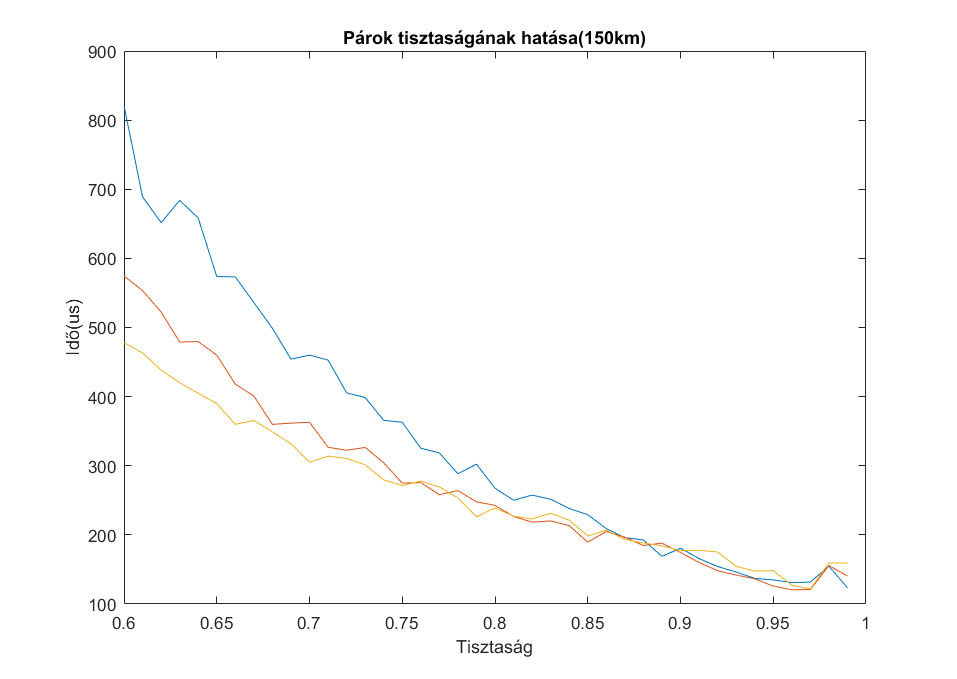
\includegraphics[width=120mm,keepaspectratio]{fidtest150}
\caption[Tisztaság hatása 150]
{Tisztaság változtatásának hatása 150 km-en.\\ 
Kék, piros, sárga vonalak: 4, 8, 16 szegmensből álló rendszerekhez tartozó adatok.\\}
\end{figure}
\begin{figure}[H]
\centering
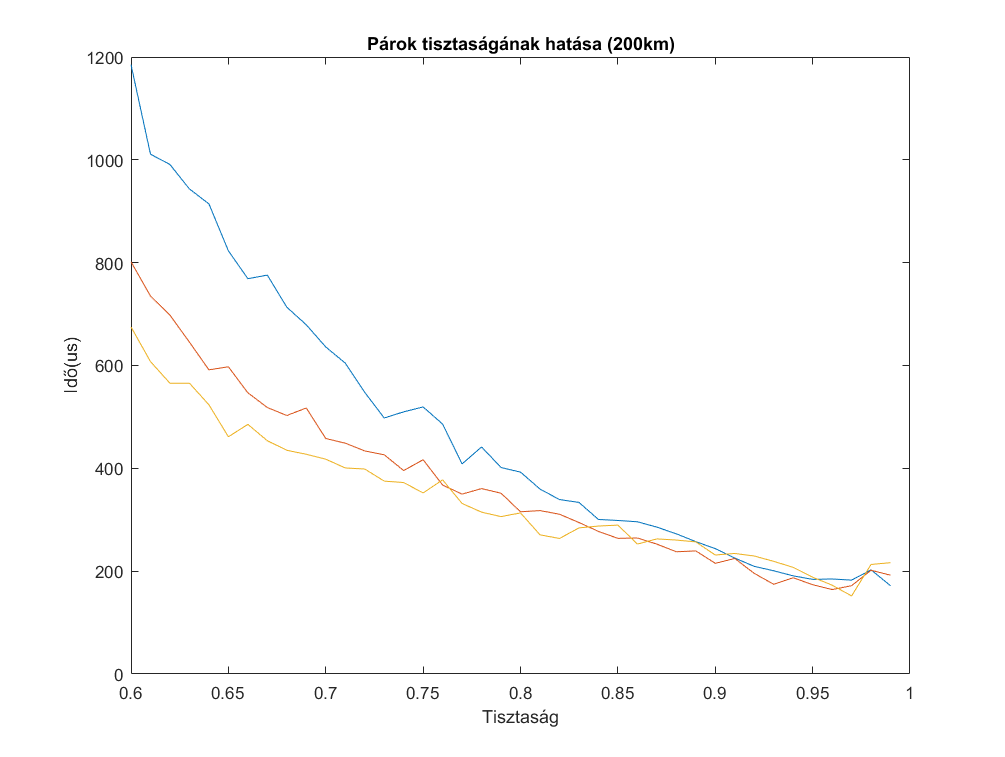
\includegraphics[width=120mm,keepaspectratio]{fidtest200}
\caption[Tisztaság hatása 200]
{Tisztaság változtatásának hatása 200 km-en.\\ 
Kék, piros, sárga vonalak: 4, 8, 16 szegmensből álló rendszerekhez tartozó adatok.\\}
\end{figure}
\begin{figure}[H]
\centering
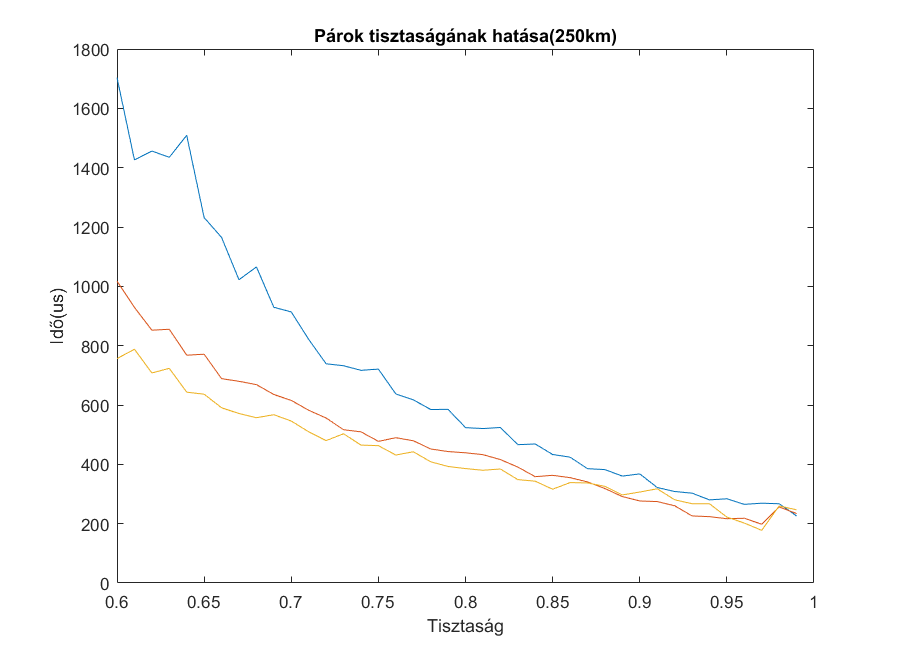
\includegraphics[width=120mm,keepaspectratio]{fidtest250}
\caption[Tisztaság hatása 250]
{Tisztaság változtatásának hatása 250 km-en.\\ 
Kék, piros, sárga vonalak: 4, 8, 16 szegmensből álló rendszerekhez tartozó adatok.\\}
\end{figure}
Az eredményekből látható, hogy minél kisebb a kezdeti tisztaság, az átviteli sebesség annál erősebben csökken. Megfigyelhető továbbá, a több szegmensből álló rendszerek növekvő előnye a kisebb értékek esetén. Egy megfontolandó technikai korlát, hogy a legtöbb tisztító eljárás 0.5-ös tisztaság alatt nem működik, emiatt arra az értékre egy abszolút alsó határként is tekinthetünk.

\subsection{Tisztító stratégiák}
Az elvégzendő tisztítások sorrendje, valamint a tisztított párok párosításának módja is hatással lehet a teljesítményre. Az eddigiekben úgynevezett ``greedy bottom up'' eljárás szerint végeztem el az egyes lépéseknél a tisztítást, ami a egyszerűen annyit jelent, hogy minden egyes tisztítási lépésben először a kisebb tisztaságú párokat tisztítom egymással, valamint az összes rendelkezésre álló tisztítható párt tisztítom. Ezen annyit változtattam, hogy egy ilyen tisztítási lépés akkor ütemeződik csak, ha a szabad memóriák száma egy adott küszöb alá kerül (fel kell szabadítani, hogy fogadhatóak legyenek az új párok). A most vizsgált másik tisztítási ütemezés a ``greedy top down''. Ebben mindig a nagyobb tisztaságú párokat tisztítjuk egymással, így haladva végig a rendelkezésre álló halmazon.
\begin{figure}[H]
\centering
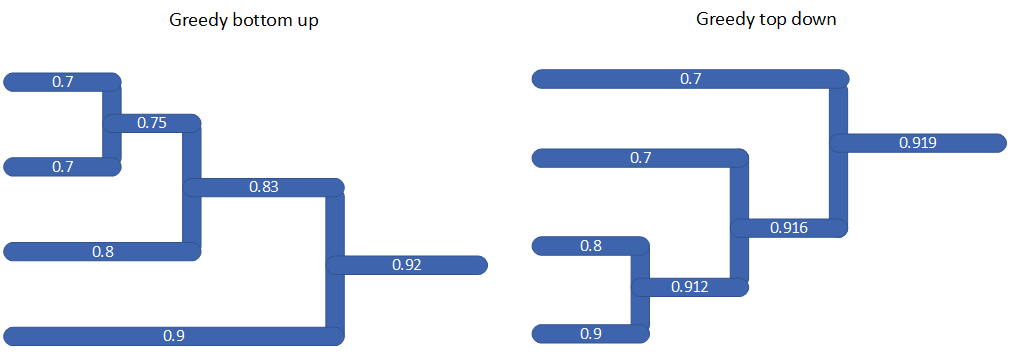
\includegraphics[width=120mm,keepaspectratio]{purifprots}
\caption[Tisztító stratégiák]
{``greedy bottom up'' és ``greedy top down'' tisztító stratégiák.\\
Az ábrán feltételezzük, hogy az egyes tisztító lépések sikeresek, valamint a keletkező új tisztaságok csak személtetésül szolgálnak, ezek pontos értéke a valóságban nagyban függ az alkalmazott tisztító eljárástól, valamint a használt párok pontos állapotától is.}
\end{figure}
Az e két protokoll közti különbségeket 150km-es távon vizsgáltam.
A kapott eredmények:
\begin{figure}[H]
\centering
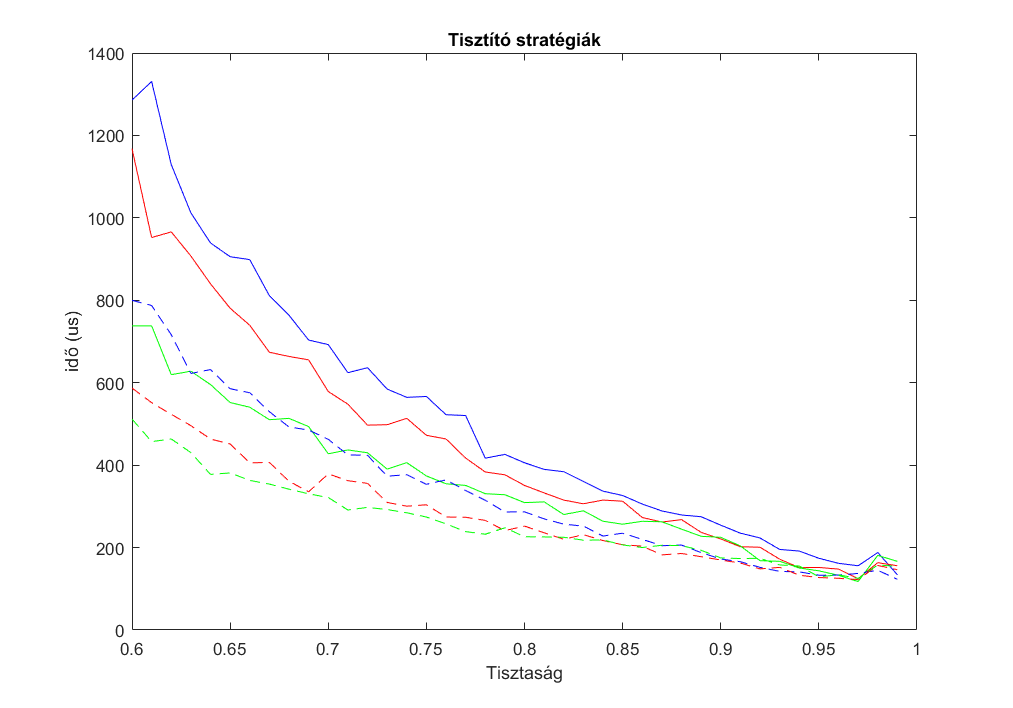
\includegraphics[width=120mm,keepaspectratio]{prottest}
\caption[Tisztító stratégiák]
{A két ismertetett stratégia teljesítményei 150 km-es távolságon \\
Kék, piros, zöld sima vonal: greedy top down 4,8 és 16 szegmenses rendszerekre. \\
Kék, piros, zöld szaggatott vonal: greedy bottom up 4,8 és 16 szegmenses rendszerekre.
}
\end{figure}
A ``greedy bottom up'' előnye látszik. Ennek egyik oka az alkalmazott tisztító eljárás azon tulajdonsága, hogy a sikeresség esélye függ a felhasznált párok tisztaságától. Így a top down filozófiát követve a nagy tisztaságú párjainkat többször párosítjuk össze kisebb tisztaságúakkal, ezáltal összességében jobban kockáztatva ezen már tisztább állapotok elvesztését. A bottom up sorrendet követve viszont először mindig a koszosabb párokat használjuk el, ezáltal az értékesebb állapotokat már csak az így szerzett nagyobb tisztaságúakkal párosítjuk, ami kevésbé kockázatos.
\subsection{Tisztasági előírások}
Az előzőekben minden Bell-mérés végrehajtásához előfeltétel volt, hogy a mérésben résztvevő párok legalább 0.98-as tisztaságúak legyenek. Ezt módosítottam úgy, hogy a 0.98-as előírás csak a protokoll két végpontja között legyen érvényes, a köztes állomások az új 0.9-es határértéket használják. 

\begin{figure}[H]
\centering
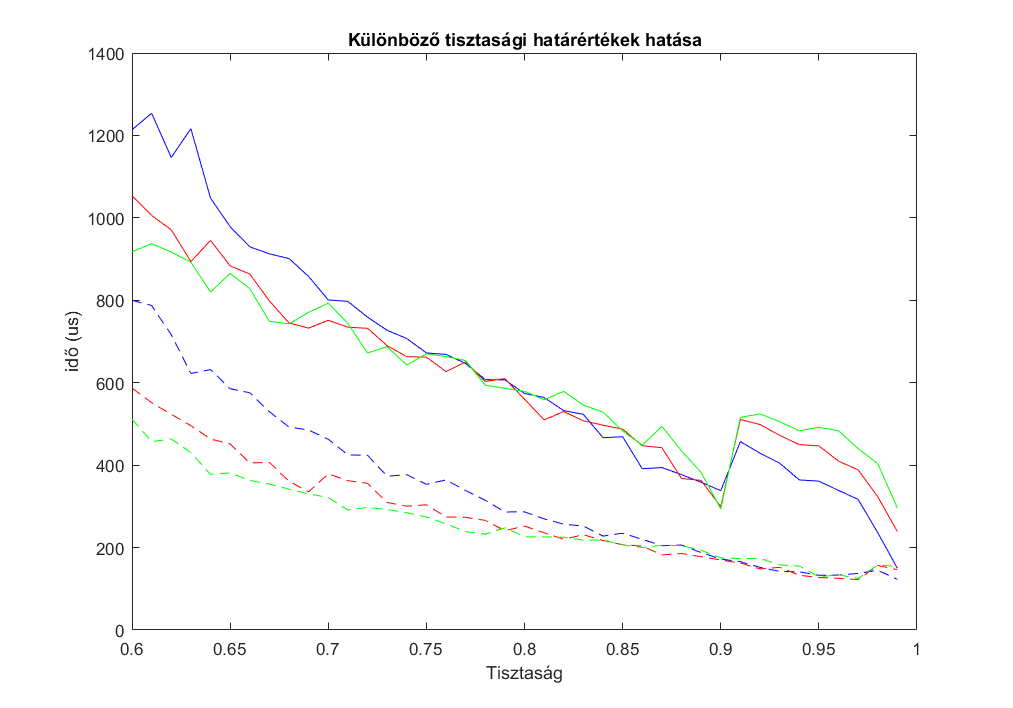
\includegraphics[width=120mm,keepaspectratio]{lowtarget}
\caption[Határérték csökkentése]
{Tisztasági előírás csökkentésének hatása150 km-es távolságon \\
Kék, piros, zöld sima vonal: csökkentett határértékkel működő rendszer 4,8 és 16 szegmens esetén. \\
Kék, piros, zöld szaggatott vonal: eredeti határértékkel működő rendszer 4,8 és 16 szegmens esetén.
}
\end{figure}

Amennyiben nem tiszta állapotokon végzünk Bell-mérést, a mérés utáni állapot tisztaságáról csak azt tudhatjuk, hogy a két kezdeti állapot tisztaságának szorzatánál nem kisebb. Ebből következik, hogy a koszosabb állapotokon végzett mérés a keletkező új pár állapotát csak tovább rontja, amit utána megint tisztítani kell. Nem megfelelő határérték esetén (pl.: < ~0.7) az is előfordulhat, hogy az alkalmazott tisztító eljárás már nem képes a Bell-mérés utáni állapot tisztítására. Szimulációs példámban látható, hogy a határérték egy kisebb változtatása is már jelentősebb romláshoz vezethet. Ugyanakkor ügyelni kell arra is, hogy ez a határérték ne legyen túl magas se, mivel a tisztító eljárások hatékonysága a teljesen tiszta állapotot közelítve romlik.

\section{Egyéb megfontolandó paraméterek}
\subsection{Protokoll indulása}
Az előzőekben kizárólag a hosszabb működés alatti átlagteljesítményt vizsgáltam, azonban meg kell említeni, hogy a rendszerek rendelkeznek egy úgymond telítődési idővel is ami indulásnál az egyes állomások kezdetben üres memóriáinak megfelelő állapotú párokkal való feltöltődésének ideje. Ennek szemléltetésére vizsgáltam a következőkben az indulástól számított első néhány sikeres megosztásig eltelt időt.
\begin{figure}[H]
\centering
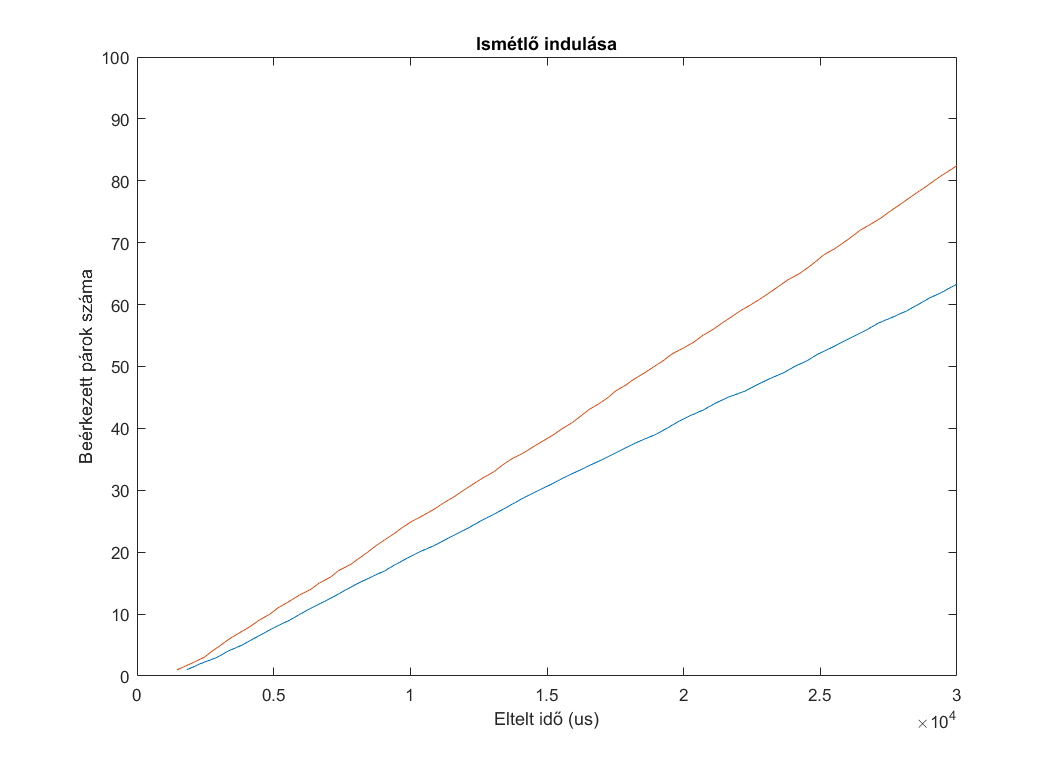
\includegraphics[width=120mm,keepaspectratio]{repstart}
\caption[Beérkezett párok indulás után]
{Beérkezett párok indulás után 150 km-es távolságnál:\\
Kék vonal: 4 szegmenses ismétlő indulása.\\
Piros vonal: 8 szegmenses  ismétlő indulása.
}
\end{figure}
A protokoll indulásánál az első pár beérkezésére többet kell várni, mint később az egyes párok között. A rendszernek ugyanis itt teljesen üres állapotból meg kell várnia a különböző műveletek elvégzése előtt, amíg a memóriák a megfelelő állapotokkal feltelnek. (A telítődés a későbbiekben a műveletekkel párhuzamosan történik.) Ez után a telítődés után már az idővel egyenesen arányosan nő a megosztott párok száma.
\subsection{Kvantumos memóriák}
Eddig az egyes állomásokon a biteket tároló memóriákat ideálisnak tekintettük, azonban a való életben ezek korántsem azok. Határaik és tökéletlenségeik komoly limitáló tényezőt jelenthetnek. A legjobb tárolási minőségre, valamint a legnagyobb tárolási időre, a végpontokban van szükség, mivel az itt tárolt bitek állapotának fent kell maradni mialatt az összes hozzájuk tartozó mérést elvégezzük. Ennek a szükséges maximális időnek az alakulását vizsgálom az első (4.2. ábra) szimulációs összehasonlítás eredményeinél.
\begin{figure}[H]
\centering
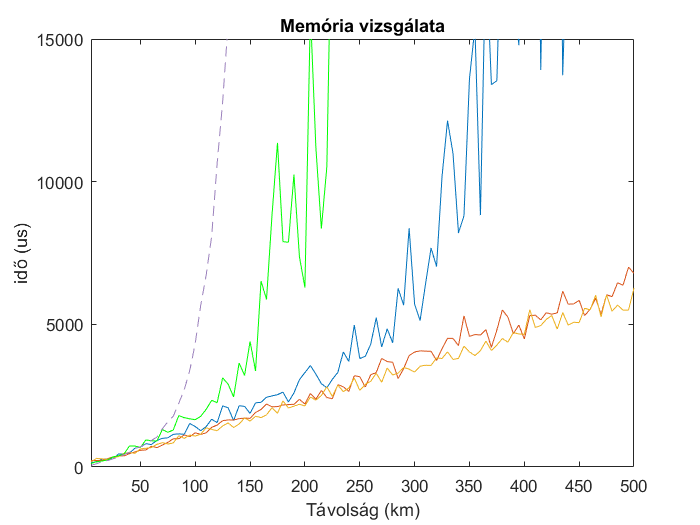
\includegraphics[width=120mm,keepaspectratio]{mems}
\caption[Párok memóriában töltött ideje]
{Párok memóriában töltött ideje:\\
Az y tengelyen az egy pár memóriában töltött átlagos idejét mérjük.\\
Lila szaggatott vonal:egyszerű csatorna.\\
Zöld, kék, piros, narancs vonalak: 2, 4, 8 valamint 16, köztes létrehozó állomásból álló ismétlő rendszerek.\\
Alsó fekete pontozott vonal: 8 köztes állomásból álló rendszer teljes tisztaság esetén.\\
A szimulációs beállítások a 4.2.-es esethez használtakkal egyezőek.
}
\end{figure}
A memóriában töltött idő szórása jelentősen nagyobb mint az átvitel vizsgálatának esetében, 200 esetből történő átlagolás esetén is észrevehető. A függvények jellege nem változott, viszont látszik, hogy az átviteli sebesség többszörösét töltik a párok a rendszerben valamint, hogy az egyszerű csatorna esetén is számolni kell ezzel a tényezővel, amennyiben a végpontok között tisztítás szükséges.


\section{Az alkalmazott modell korlátai}
Mivel az előző vizsgálatokat egy általánosított modellen végeztem, az ebből származó eredmények, bár egy becslést adhatnak,  is erre a modellre igazak. Egy konkrét megvalósítás pontos szimulációjához megfontolandóak további változtatások. Az alkalmazandó memória pontos ismeretében a maximum tárolási idő meghatározható. Ennek ismeretében a szimuláció során az ezt meghaladó tárolt párokat a memóriából törölhetjük, aminek hatására az átvitel tovább változhat. Az alkalmazandó csatorna pontos ismeretében (kábel, szabadtéri, átküldendő adat hordozója stb...) lehet pontosabban vizsgálni a csatorna által okozott tisztaságromlás hatását különböző távolságok esetén. Az általánosított modell továbbá nem számol az állomásokon elvégzett műveletek tökéletlenségével, ami további korlátot jelenthet a sebességre nézve. Az alkalmazott fizikai megvalósításokból származhatnak kifejezetten technológiafüggő egyéb paraméterek is. 

\chapter{Összefoglalás}

Dolgozatomban megvizsgáltam a kvantumkommunikáció jelenkori határait, általa támasztott kihívások, valamint ezek egy lehetséges megoldását kvantum összefonódás megosztás segítségével. A téma áttekintése, valamint a szükséges elméleti bevezető és a jelenség ismertetése után, az ezt felhasználó kvantum ismétlő protokollt, és ennek megvalósításait vizsgáltam. A protokoll sajátosságainak, valamint az általa támasztott technológiai feltételek vizsgálatára készítettem egy általános kvantum ismétlő protokoll szimulációjára képes programot, melynek segítségével ezen vizsgálatokat elvégeztem. A program által szolgáltatott eredmények az elméleti modelleknek megfelelőek. Összességében megállapítható a kvantum ismétlők előnye az egyszerű csatornához képest, valamint nagyobb távolságok esetére való megvalósíthatóságuk. Ahhoz azonban, hogy a való életben is széleskörűen gazdaságos megoldást kínálhassanak a jelen problémáira, a protokollt alkotó egyes elemek (memória, mérések) további fejlődésére van szükség.
